\documentclass[12pt]{article}
%	options include 12pt or 11pt or 10pt
%	classes include article, report, book, letter, thesis
\usepackage{amsmath} 
\usepackage{amstext}  
\usepackage{graphicx}
\usepackage{natbib}

   

\title{This is the title}
\author{Author One \\ Author Two}
\date{29 February 2004}

\begin{document}
\maketitle

% terjemahan :

\section{Energy-Based Model (EBM)}
EBM mengaitkan sebuah energi skalar pada setiap konfigurasi variable yang diinginkan. Proses learning bertujuan untuk memodifikasi fungsi energi sehingga bentuknya memiliki  sifat yang diinginkan. Sebagai contoh, misalnya diinginkan sebuah bentuk konfigurasi yang memiliki energi yang rendah, maka model probabilistik dari EBM didifinisikan sebagi distribusi probabilitas melalui fungsi energi sebagi berikut:
\begin{equation}
p(x) = \frac {e^{-E(x)}} {Z}.
\end{equation}

Z adalah faktor normalisasi yang disebut sebagai fungsi partisi untuk menganalogikan dengan sistem fisika.

\[Z = \sum_x e^{-E(x)}\]

EBM bisa dilatih dengan cara melakukan (stochastic) gradient descent pada negative log-likelihood (NLL)-nya secara empiris pada data training. Adapun untuk logistic regression akan didifinisikan terlebih dahulu log-likelihood $\mathcal{L}(\theta, \mathcal{D})$ dan fungsi loss-nya sebagai NLL $\ell (\theta, \mathcal{D})$ sebagai berikut:

\[\mathcal{L}(\theta, \mathcal{D}) = \frac{1}{N} \sum_{x^{(i)} \in
\mathcal{D}} \log\ p(x^{(i)})\]
\[\ell (\theta, \mathcal{D}) = - \mathcal{L} (\theta, \mathcal{D})
\]

Menggunakan stochastic gradient $-\frac{\partial  \log p(x^{(i)})}{\partial
\theta}$, dimana $\theta$ adalah parameter dari modelnya.

\subsection{EBM dengan Hidden Units}

Pada banyak kasus, sampel $x$ biasanya tidak terobservasi secara penuh, atau akan ditambahkan varibel yang tidak teobservasi secara langsung yang disebut dengan hidden unit, dimana hal ini berguna untuk meningkatkan ekspresivitas dari model. Sehingga dikenalkan bagian yang terobservasi disini dilambangkan dengan $x$, dan sebuah bagian yang tersembunyi $h$. Sehingga bisa ditulis sebagai:
\begin{equation}
P(x) = \sum_h P(x,h) = \sum_h \frac{e^{-E(x,h)}}{Z}.
\end{equation}

Pada kasus ini, untuk melakukan pemetaan rumus yang mirip dengan rumus (1), akan dikenalkan notasi (yang merupakan inspirasi dari fisika) yaitu free energy $\mathcal{F}(x)$, yang didifinisikan sebagai berikut:

\begin{equation}
\mathcal{F}(x) = - \log \sum_h e^{-E(x,h)}
\end{equation}
Sehingga bisa diturunkan sebagai :
\[P(x) = \frac{e^{-\mathcal{F}(x)}}{Z} \text{ dengan } Z=\sum_x e^{-\mathcal{F}(x)}.\]

Data dari gradien NLL kemudian memiliki bentuk yang menarik yaitu:
\begin{equation}
- \frac{\partial  \log p(x)}{\partial \theta}
 = \frac{\partial \mathcal{F}(x)}{\partial \theta} -
       \sum_{\tilde{x}} p(\tilde{x}) \
           \frac{\partial \mathcal{F}(\tilde{x})}{\partial \theta}.
\end{equation}

Gradien tiatas memiliki dua istilah, dimana hal tersebut mereferensikan pada fase positif dan fase negatif. Istilah positif dan negatif ini tidak merujuk pada tanda (positif/negatif)  persamaan, akan tetapi merefleksikan efek pada kepadatan probabilitas yang didefinisikan oleh model. Istilah pertama, menambah probabilitas data training (dengan cara mengurangi free energy yg berhubungan), sedangkan istilah kedua mengurangi probabilitias sampel yang digenerasi oleh model.\\

Biasanya sulit untuk menentukan gradien secara analitis, oleh karena berhubungan dengan komputasi dari $E_P [ \frac{\partial \mathcal{F}(x)} {\partial \theta} ]$. Dikarenakan hal ini merupakan ekspektasi semua kemungkinan konfigurasi input $x$ (pada distribusi $P$ yang dibentuk oleh model).\\
Oleh karena itu, langkah pertama agar bisa dikomputasi secara analitis maka dilakukan estimasi ekspektasi menggunakan jumlah yang pasti dari sampel pada model. Sampel digunakan untuk mengestimasi gradien dari fase negatif yang direferensikan sebagai partikel negatif, dimana disimbolkan sebagai $\mathcal{N}$. Kemudian, gradien bisa ditulis sebagai : 

\begin{equation}
- \frac{\partial \log p(x)}{\partial \theta}
 \approx
  \frac{\partial \mathcal{F}(x)}{\partial \theta} -
   \frac{1}{|\mathcal{N}|}\sum_{\tilde{x} \in \mathcal{N}} \
   \frac{\partial \mathcal{F}(\tilde{x})}{\partial \theta}.
\end{equation}
Dimana secara ideal, elemen seperti $\tilde{x}$ dari $\mathcal{N}$ disampel menurut $P$ (sebagai contoh adalah menggunakan teknik sampling Monte-Carlo). Dengan rumus diatas, secara praktis hampir bisa melakukan algoritma stochastic, hanya saja partikel negatif $\mathcal{N}$ belum bisa diekstraksi. Oleh karena itu, pada literatur dengan metode Markov Chain Monte Carlo, sangat bagus digunakan pada model Restricted Boltzmann Machine (RBM) yang merupakan bentuk spesifik dari model EBM.

\section{Restricted Boltzmann Machines (RBM)}
Boltzmann Machines (BMs) adalah bentuk khusus dari log-linear Markov Random Field (MRF), dengan kata lain, dimana fungsi energi adalah linear pada parameter bebasnya. Agar membuat BM cukup bisa merepresentasikan distribusi yang kompleks(dengan kata lain, berangkat dari setting parameter yang terbatas kepada non paramter), diasumsikan bahwa beberapa variabel tidak terobserbasi sehingga disebut hidden. Dengan memiliki variabel hidden, bisa dilakukan peningkatan kapasitas model dari BM. RBM, selanjutnya membuat BM yang terbatas pada variabel tanpa koneksi visibel-visibel dan hidden-hidden. Seperti pada gambar \ref{fig:rbm}\\
\begin{figure}
	\centering
	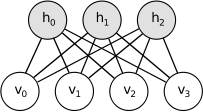
\includegraphics[width=0.3\textwidth]
		{pics/rbm.png}
	\caption{Grafik yang Menggambarkan RBM}
	\label{fig:rbm}
\end{figure}

Fungsi energi $E(v,h)$ pada RBM didefinisikan sebagai persamaan \ref{eq:rbm1}.

\begin{equation}
E(v,h) = - b'v - c'h - h'Wv
\label{eq:rbm1}
\end{equation}

Dimana $W$ merepresentasikan bobot yang terkoneksi antara unit hidden dan visible dan $b$, $c$ adalah bias dari visible dan hidden secara berurutan.\\

Hal ini bisa diterjemahkan dalam bentuk persamaan energi bebas $\mathcal{F}(v)$ seperti dibawah:
\[\mathcal{F}(v)= - b'v - \sum_i \log \sum_{h_i} e^{h_i (c_i + W_i v)}.\]
Dikarenakan struktur RBM yang spesifik, visibel dan hidden adalah independen secara bersyarat antara satu dengan lainnya. Dengan menggunakan sifat tersebut, maka dapat dituliskan :

\[p(h|v) = \prod_i p(h_i|v)\]
\[p(v|h) = \prod_j p(v_j|h).\]

\subsection{RBMs yang Menggunakan Unit Biner}

Kasus umum jika menggunakan unit biner (dimana $v_j$ dan $h_i \in
\{0,1\})$, yang didapat dari persamaan (6) dan (2), versi probabilistik dari fungsi aktivasi neuron adalah sebagai berikut:

\begin{equation}
P(h_i=1|v) = sigm(c_i + W_i v)
\end{equation}

\begin{equation}
P(v_j=1|h) = sigm(b_j + W'_j h)
\end{equation}

Selanjutnya, energi bebas dari RBM dengan unit biner, disederhanakan menjadi persamaan:

\begin{equation}
\mathcal{F}(v)= - b'v - \sum_i \log(1 + e^{(c_i + W_i v)}).
\end{equation}

\subsection{Update Persamaan dengan Unit Biner}

Menghubungkan persamaan (5) dengan (9), didapatkan gradien log-likelihood untuk RBM dengan unit biner sebagai berikut:

\begin{equation}
- \frac{\partial{ \log p(v)}}{\partial W_{ij}} =
    E_v[p(h_i|v) \cdot v_j]
    - v^{(i)}_j \cdot sigm(W_i \cdot v^{(i)} + c_i)
\end{equation}

\[-\frac{\partial{ \log p(v)}}{\partial c_i} =
    E_v[p(h_i|v)] - sigm(W_i \cdot v^{(i)})\]
\[-\frac{\partial{ \log p(v)}}{\partial b_j} =
    E_v[p(v_j|h)] - v^{(i)}_j\]


\section{Sampling pada RBM}

Sampel dari $p(x)$ bisa didapat dengan menjalankan Markov chain sampai konvergen dengan menggunakan gibbs samping sebagai operator transisi. \\

Gibbs sampling dari join variable random sebanyak $N$ dari $S=(S_1, ... , S_N)$ merupakan urutan sebanyak $N$ sampling dari sub-steps dalam bentuk $S_i \sim p(S_i | S_{-i})$ dimana $S_{-i}$ berisi $N-1$ variabel random lain didalam $S$ tetapi diluar $S_i$.

Untuk RBM, $S$ berisi himpunan dari visible dan hidden unitnya. Akan tetapi, dikarenakan unit ini dipenden secara kondisional, maka salah satunya bisa dilakukan gibbs sampling. Pada setting disini, unit visible disampel secara simultan given nilai fix dari hidden unitnya. Demikian sebaliknya, hidden unitnya disampel secara simultan given unit visibelnya.Sehingga satu langkah Markov chain adalah sebagai berikut: 

\[h^{(n+1)} \sim sigm(W'v^{(n)} + c)\] 
\[v^{(n+1)} \sim sigm(W h^{(n+1)} + b),\]

Dimana $h^{(n)}$ menunjik pada himpunan semua hidden unit pada nilai yang ke-$n$ langkah dari Markov chain. Yang artinya adalah sebagai contoh, $h^{(n+1)}_i$ adalah secara random dipilih antara 1 (versus 0) dengan nilai probabilitas $sigm(W_i'v^{(n)} + c_i)$, demikian juga, $v^{(n+1)}_j$ adalah dipilih secara random antara 1 (versus 0) dengan probabilitas $sigm(W_{.j} h^{(n+1)} + b_j)$.

Hal ini seperti digambarkan pada gambar \ref{fig:markov_chain}
\begin{figure}
	\centering
	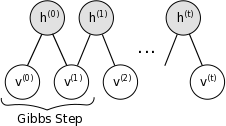
\includegraphics[width=0.3\textwidth]
		{pics/markov_chain.png}
	\caption{Gibbs Sampling}
	\label{fig:markov_chain}
\end{figure}


Oleh karena $t \rightarrow \infty$, maka sampel $(v^{(t)}, h^{(t)})$ bisa dipastikan akan akurat dalam mensampel $p(v,h)$.

Secara teori, tiap parameter diupdate pada proses learning dibutuhkan satu rantai tersebut untuk konvergen. Akan tetapi hal ini sangat mahal komputasinya. Sehingga banyak diajukan algoritma untuk melatih RBM agar sampel $p(v,h)$ efisien, disaat proses learningnya.

\section{Contrastive Divergence (CD-k)}

Contrastive Divergence(CD) menggunakan trik untuk mempercepat proses sampling: \\


Contrastive Divergence uses two tricks to speed up the sampling process:
Dikarenakan yang diinginkan adalah $p(v) \approx p_{train}(v)$ (distribusi data yang asli), initialisasi  Markov chain dengan contoh data training (dimana, berasal dari distribusi yang mendekati $p$, pada distribusi final dari $p$). CD tidak menunggu rantai untuk konvergen. Sampel didapatkan setalah langkah ke-$k$ dari Gibbs sampling. Pada prakteknya, $k=1$ secara mengejutkan sudah menghasilkan hasil yang baik.\\

\section{Persistent CD}

Persistent CD (P-CD) [Tieleman08] menggunakan pendekatan lain untuk mensampling $p(v,h)$. Hal ini bergantung hanya pada Markov chain tunggal, yang memiliki kondisi yang persisten (dimana, tidak melakukan restart chain pada setiap sampel yang terobservasi). Pada setiap umpdate parameter, akan di ekstraksi sampel baru dengan penjalankan chain pada langkah ke-$k$. Kondisi chain akan dipertahankan pada update selanjutnya.\\
Intuisinya adalah jika update parameternya cukup kecil dibaningkan dengan rate campuran dari Markov Chain, maka hal ini bisa mengejar perubahan modelnya.

\section{Deep Belief Networks}

Hinton menunjukkan bahwa RBM bisa dijajar dan dilatih secara greedy untuk membentuk sebuah jaringan yang dinamakan dengan Deep Belief Network (DBN). DBN adalah model grafis dimana bisa melakukan learning untuk mengekstraksi representasi hirarki yang mendalam (deep) dari data training. Hal ini memodelkan distribusi gabungan antara vektor x sebagai observer dan $\ell$ layer hidden $h^k$ sebagai berikut:

\begin{equation}
P(x, h^1, \ldots, h^{\ell}) = \left(\prod_{k=0}^{\ell-2} P(h^k|h^{k+1})\right) P(h^{\ell-1},h^{\ell})
\end{equation}

Dimana $x=h^0, P(h^{k-1} | h^k)$ adalah distribusi kondisional untuk unit visible dikondisikan pada unit hidden pada level $k$ dan  $P(h^{\ell-1}, h^{\ell})$ adalah distribusi gabungan visible-hidden pada level teratas dar RBM. Seperti diilustrasikan pada gambar \ref{fig:dbn3}.

\begin{figure}
	\centering
	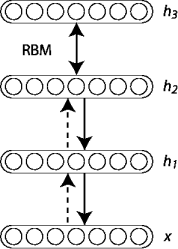
\includegraphics[width=0.3\textwidth]
		{pics/DBN3.png}
	\caption{Arsitektur Deep Believe Network (DBN) yang merupakan gabungan dari RBM}
	\label{fig:dbn3}
\end{figure}


Prinsip dari greedy layer-wise unsupervised training bisa di aplikasikan pada DBN dengan RBM sebagai bagian pada tiap layernya [hinton] [bengio]. Pada prinsipnya prosesnya adalah sebagai berikut:
\begin{enumerate}
\item Latih layer pertama ssebagai RBM yang memodelkan input $x = h^{(0)}$ sebagai visible layernya.
\item Gunakan layer pertama untuk mendapatkan representasi input yang digunakan sebagai data untuk layer kedua. Ada dua solusi yang sama. Representasi ini bisa dipilih sebagai rata-rata dari aktivasi $p(h^{(1)}=1|h^{(0)})$ atau sampel dari $p(h^{(1)}|h^{(0)})$.
\item Train layer kedua sebagai RBM dengan mengambil data transformasi (sampel atau rata-rata aktivasi) sebagai training (untuk layer visible dari RBM tersebut).
\item Iterasikan (2 dan 3) untuk semua layer yang diinginkan, setiap waktu dengan mempropagasikan keatas antara sampel atau nilai rata-ratanya.
\item Fine-tune semua parameter dari arsitektur dengan log-likelihood DBN atau dengan kriteria secara supervised setelah menambahkan layer supervised untuk memprediksikan kelas, sebagai contoh misalnya layer logistic regression.
\end{enumerate}

Pada kasus ini, akan difokuskan pada fine-tuning dengan melakukan gradien descent menggunakan klassifier logistic regression dimana digunakan untuk mengklasifikasikan input x berdasar pada output dari hidden layer $h^{(l)}$ dari DBN. Fine-tune kemudian dilakukan melalui gradien descent dari NLL fungsi costnya. Dikarenakan gradien secara supervised adalah hanya non-null untuk bobot dan bias pada hidden layer pada tiap-tiap layer, maka prosedur ini serupa dengan menerapkan initialisasi parameter dari arsitektur MLP yang deep dengan bobot dan bias dari hidden layer yang didapat pada proses training unsupervised diatas.

\section{Alasan Melakukan Training Secara Greedy Layer-Wise}

Algoritma training deep learning secara greedy layer-wise terbukti bisa bekerja dengan baik, sebagai contoh 2 layer DBN dengan hidden layer $h^{(1)}$ dan $h^{(2)}$ dengan parameter bobot berurutan adalah $W^{(1)}$ dan $W^{(2)}$, \citep{hinton2006reducing} maka $\log
p(x)$ bisa ditulis sebagai:
\begin{equation}
\begin{aligned}
\log p(x) = &KL(Q(h^{(1)}|x)||p(h^{(1)}|x)) + H_{Q(h^{(1)}|x)} + \\
            &\sum_h Q(h^{(1)}|x)(\log p(h^{(1)}) + \log p(x|h^{(1)})).
\end{aligned}
\label{eq:equ2}
\end{equation}

$KL(Q(h^{(1)}|x) || p(h^{(1)}|x))$ merepresentasikan KL divergence antara posterior $Q(h^{(1)}|x)$ dari RBM pertama jika hal ini sendirian, dan probabilitas $p(h^{(1)}|x)$ untuk layer sayng sama tapi didifinisikan oleh keseluruhan DBN (sebagai contoh, perhitungan prior $p(h^{(1)},h^{(2)}$) didefinisikan sebagai top-level RBM). $H_{Q(h^{(1)}|x)}$ adalah entropy dari distribusi $Q(h^{(1)}|x)$.\\
Hal ini bisa ditunjukkan bahwa jika diinitialisasi kedua layer hidden sehingga $W^{(2)}={W^{(1)}}^T, Q(h^{(1)}|x)=p(h^{(1)}|x)$ dan KL divergence nya adalah null. Maka jika di lakukan learning pada level awal RBM dan kemudian parameter $ W^{(1)}$ dibuat tetap, kemudian dilakukan optimasi pada persamaan \ref{eq:equ2} terhadap $W^{(2)}$ bisa meningkatkan likelihood dari $p(x)$.
Jika diisolasi hanya pada $W^{(2)}$ sehinggi didapatkan:

\[\sum_h Q(h^{(1)}|x)p(h^{(1)})\]

Melakukan optimasi persamaan ini dengan memperhatikan jumlah $W^{(2)}$ training pada tingkat RBM selanjutnya, menggunakan output dari $Q(h^{(1)}|x)$ sebagai distribusi training untuk RBM yang pertama.

Breakthrough in Learning Deep Architectures
Before 2006, attempts at training deep architectures failed: training a deep supervised feedforward neural network tends to yield worse results (both in training and in test error) then shallow ones (with 1 or 2 hidden layers).

Three papers changed that in 2006, spearheaded by Hinton’s revolutionary work on Deep Belief Networks (DBNs):

Hinton, G. E., Osindero, S. and Teh, Y., A fast learning algorithm for deep belief nets Neural Computation 18:1527-1554, 2006
Yoshua Bengio, Pascal Lamblin, Dan Popovici and Hugo Larochelle, Greedy Layer-Wise Training of Deep Networks, in J. Platt et al. (Eds), Advances in Neural Information Processing Systems 19 (NIPS 2006), pp. 153-160, MIT Press, 2007
Marc’Aurelio Ranzato, Christopher Poultney, Sumit Chopra and Yann LeCun Efficient Learning of Sparse Representations with an Energy-Based Model, in J. Platt et al. (Eds), Advances in Neural Information Processing Systems (NIPS 2006), MIT Press, 2007
The following key principles are found in all three papers:

Unsupervised learning of representations is used to (pre-)train each layer.
Unsupervised training of one layer at a time, on top of the previously trained ones. The representation learned at each level is the input for the next layer.
Use supervised training to fine-tune all the layers (in addition to one or more additional layers that are dedicated to producing predictions).
The DBNs use RBMs for unsupervised learning of representation at each layer. The Bengio et al paper explores and compares RBMs and auto-encoders (neural network that predicts its input, through a bottleneck internal layer of representation). The Ranzato et al paper uses sparse auto-encoder (which is similar to sparse coding) in the context of a convolutional architecture. Auto-encoders and convolutional architectures will be covered later in the course.

Since 2006, a plethora of other papers on the subject of deep learning has been published, some of them exploiting other principles to guide training of intermediate representations. See Learning Deep Architectures for AI for a survey.

\end{document}
